\documentclass[11pt,a4paper]{article}

\usepackage{graphicx}
\graphicspath{{Images/}{./}}

\usepackage[hang,bottom]{footmisc}
\usepackage{adjustbox}
\usepackage{amsmath,amssymb,amsfonts,amsthm}
\usepackage{bm}
\usepackage{natbib}
\usepackage{lipsum}
\usepackage{advdate}
\usepackage{adjustbox}
\usepackage{booktabs} 
\usepackage{tikz}
\usepackage{pdfpages}
\usepackage{caption}
\usepackage{hyperref}
\hypersetup{
    colorlinks=true,
    citecolor=black,
    linkcolor=black,
    filecolor=black,
    urlcolor=black,
    pdfpagemode=FullScreen,
}

\setlength{\textheight}{23.5cm}
\setlength{\topmargin}{-1.05cm}
\setlength{\textwidth}{6.5in}
\setlength{\oddsidemargin}{-0.5cm}

\newtheorem{proposition}{Proposition}
\newtheorem{lemma}{Lemma}
\newtheorem{assumption}{Assumption}
\newtheorem{definition}{Definition}

\begin{document}

\title{Aspirations in the Air: Effect of Development\\ Schemes on AQI\\[0.4em]
\large Evidence from a Spatial RD in India}
\author{
Aayushi Agarwal \and
Bhaskar Agarwal \and
Gaurav Banerjee \and
Nandish Patel
}
\date{\today}
\maketitle

\section{Introduction}
Development is a double-edged sword. On one hand, it promises better
infrastructure, improved livelihoods, and economic growth. On the other, it
often comes with environmental costs that aren't immediately visible but deeply
consequential. In India, where massive development schemes touch millions of
lives, understanding this trade-off isn't just an academic exercise: it's a
matter of public health. This paper asks a straightforward question: when the
government invests heavily in developing certain districts, what happens to the
air people breathe? We focus on India's Aspirational Districts Scheme, launched
in 2018 to rapidly transform 117 underdeveloped districts, and use spatial
regression discontinuity to measure its impact on PM2.5 pollution levels. What
we find challenges simple narratives about development and environment,
revealing that the answer depends critically on what kind of development
happens and where.

\section{Background}
\subsection{Motivation}
When we first started thinking about this research question, we were struck by
a simple but profound dilemma. We all want development—better roads, more
industries, improved living standards. But what if development comes at a cost
we don't often talk about? What if the very policies designed to lift people
out of poverty are also making the air they breathe more toxic? India is home
to some of the most polluted cities in the world. If you've ever visited Delhi
in winter or walked through an industrial town in the evening, you know what
we're talking about. The air feels heavy, sometimes you can even see it—a
grey-brown haze hanging over everything. This isn't just uncomfortable; it's
deadly. According to various health studies, air pollution contributes to
millions of premature deaths in India every year. But here's what made us
curious: development policies are being rolled out across hundreds of districts
in India. Some districts get these programs, others don't. What happens to air
quality in the places that receive development interventions? Does it get
better because people switch from burning wood to using clean cooking gas? Or
does it get worse because suddenly there are more construction sites, more
factories, more vehicles on newly built roads? This isn't just an academic
question. If we're going to design policies that genuinely improve people's
lives, we need to understand their full impact—not just on income or education,
but also on the environment that people live in every single day. The problem
is, it's really hard to figure out what causes what. Do districts with worse
air quality get selected for development programs? Or do development programs
themselves change air quality? We spent a lot of time thinking about how to
untangle this mess, and that's what led us to the approach we'll describe in
this paper.

\subsection{Two Ways Development Could Affect Air Quality}

As we dug deeper into this question, we realized that development could affect
air quality in completely opposite ways. Let us explain both possibilities,
because understanding these competing mechanisms is crucial to making sense of
our results.

\textbf{Mechanism I: Development Could Make Air Quality Better}

Think about a typical household in rural India. Many families still cook using
traditional stoves that burn wood, dung cakes, or crop residue. These stoves
produce a lot of smoke—not just inside the house (which is terrible for women
and children who spend time cooking), but also outside, contributing to the
overall pollution in the area. Now, imagine a development program comes in and
helps families switch to LPG gas cylinders or cleaner cooking technologies.
Suddenly, you have hundreds or thousands of households that are no longer
burning biomass every day. That should improve air quality, right? There are
other ways development might help too. Better waste management systems mean
less garbage being burned in open pits. We've seen this ourselves—in many
towns, people simply burn their trash because there's no other option.
Development programs that set up proper waste collection and disposal can
eliminate this source of pollution. Similarly, programs that teach farmers
alternatives to burning crop residue after harvest could reduce those massive
seasonal spikes in air pollution that we see in states like Punjab and Haryana.
So through this lens, development looks like it should improve air quality.
More resources mean cleaner technologies, better systems, less pollution. This
is what we call the "optimistic mechanism."

\textbf{Mechanism II: Development Could Make Air Quality Worse}

But wait—there's another story we could tell, and it's quite different.
Development often means construction. Roads being built, buildings going up,
infrastructure projects everywhere. Anyone who's lived near a construction site
knows what this means: dust everywhere, trucks rumbling by all day, diesel
generators running constantly. All of this produces pollution. Then there's
industrialization. Development programs often try to boost industrial
output—more factories, more manufacturing. These activities produce emissions.
Even if individual factories follow pollution control norms (which, let's be
honest, doesn't always happen), having more industrial activity in an area
generally means more pollution overall. And here's something we found
particularly interesting: better roads might actually increase pollution in the
short to medium term. How? Better roads mean more vehicles. Development
increases incomes, and people buy motorcycles, cars, trucks. More vehicles mean
more emissions, especially in India where emission standards aren't always
strictly enforced and many vehicles are quite old. There's also a concentration
effect. As development happens, economic activity tends to cluster in certain
areas. Urbanization increases. Instead of pollution being spread out over a
large rural area, it gets concentrated in smaller spaces where more people are
affected by it. So through this lens, development looks like it should worsen
air quality. More construction, more industry, more vehicles, more concentrated
activity. This is what we call the "pessimistic mechanism."

\textbf{So Which Is It?}

The honest answer? We don't know—and that's exactly why this research is
important! Both mechanisms make sense theoretically. Both are probably
happening simultaneously. The real question is: which effect is stronger? Does
the positive impact of cleaner cooking and better waste management outweigh the
negative impact of construction and industrialization? Or is it the other way
around? Moreover, the answer might be different in different places. A state
that emphasizes clean cooking programs might see air quality improvements. A
state that focuses heavily on infrastructure and industrial development might
see air quality deteriorate. This is fundamentally an empirical
question—something we need to measure and test, not just theorize about.

\subsection{The Aspirational Districts Scheme: Our Natural Experiment}

To answer this, we needed a situation where development happened in some places
but not others, where that difference wasn't driven by factors independently
affecting air quality. Enter "exogenous variation." In January 2018, the Indian
government launched the Aspirational Districts Scheme (ADS)—identifying 117 of
India's most underdeveloped districts for extra attention, resources, and
support. NITI Aayog managed this program, focusing on basic infrastructure,
health and nutrition, education, and agriculture with financial inclusion.
Districts were selected based on a composite deprivation index. Crucially,
these boundaries were drawn long ago, often during British colonial times.
Nobody created these boundaries anticipating the 2018 scheme. This creates a
"natural experiment." Imagine two similar villages just kilometers apart. One
falls just inside an ADS district and gets extra development attention; the
other falls just outside and doesn't. Otherwise, they're quite similar. By
comparing areas just inside ADS boundaries to areas just outside, we can
isolate the program's effect on air quality. Villages on either side should be
similar except for the intervention. This approach gives us a credible way to
answer: How does development actually affect air quality based on what happened
in these 117 districts?

\section{Methodology}
\subsection{Subdistricts Data}
A geographic RDD study by definition requires spatial data for the units of
interest. The granularity of said units for this study will be the subdistrict
level - we compare subdistricts just along a treatment border to isolate the
causal effect of the treatment (ADS). From among the several available formats
of spatial data, we have used subdistrict shapefiles (.shp) which is compatible
with most packages in the statistical software of our choice, R. To access
authentic and updated subdistrict polygons, we downloaded all India level
shapefiles from the Onlinemaps portal of SoI. It contains 4723 features, 5
fields (tehsil, district, state, shape length and shape area) and projected CRS
(Coordinate Reference System) of “LCC WGS84”.

\subsection{ADS Treatment Status}
As discussed earlier, we use the 2018 updated list of ‘Aspirational Districts’
to identify treatment status. A detailed list
containing names of all 117 districts under ADS is presented in Table 4.4. To
arrive at an indicator for treatment status, we have to generate a binary
variable in the subdistricts shape file using the list of the ‘Aspirational
Districts’. However, the list of districts provided by NITI Aayog does not have
any geo-spatial attributes. Hence, we use a fuzzy matching algorithm known as
‘Jaro Distance’ to merge data using string values (i.e., the names of the
districts). This algorithm assigns a similarity score to each string in the
master common id with all the strings in the secondary common id using the
following formula and then, the string in the secondary dataframe with the
highest similarity can be assigned to the respective string in the master
dataframe.

\begin{equation*}
\text{Similarity} =
\begin{cases}
0, & \text{if } m = 0, \\[6pt]
\dfrac{1}{3}\left(\dfrac{w_1 m}{|a|}+\dfrac{w_2 m}{|b|}+\dfrac{w_3 (m - t)}{m}\right),
& \text{otherwise.}
\end{cases}
\end{equation*}

Here, $m$ is the number of character matches, $t$ is the number of
transpositions, $|a|$ is the number of characters in string $a$ and $w_i$ are
weights summing to $3$ \cite{stringdist2023}.

After applying the algorithm, some corrections had to be made manually. Figure
\ref{fig:tut} plots the filtered subdistricts for the 27 states with
treatment status.

\begin{figure}[htbp]
    \centering
    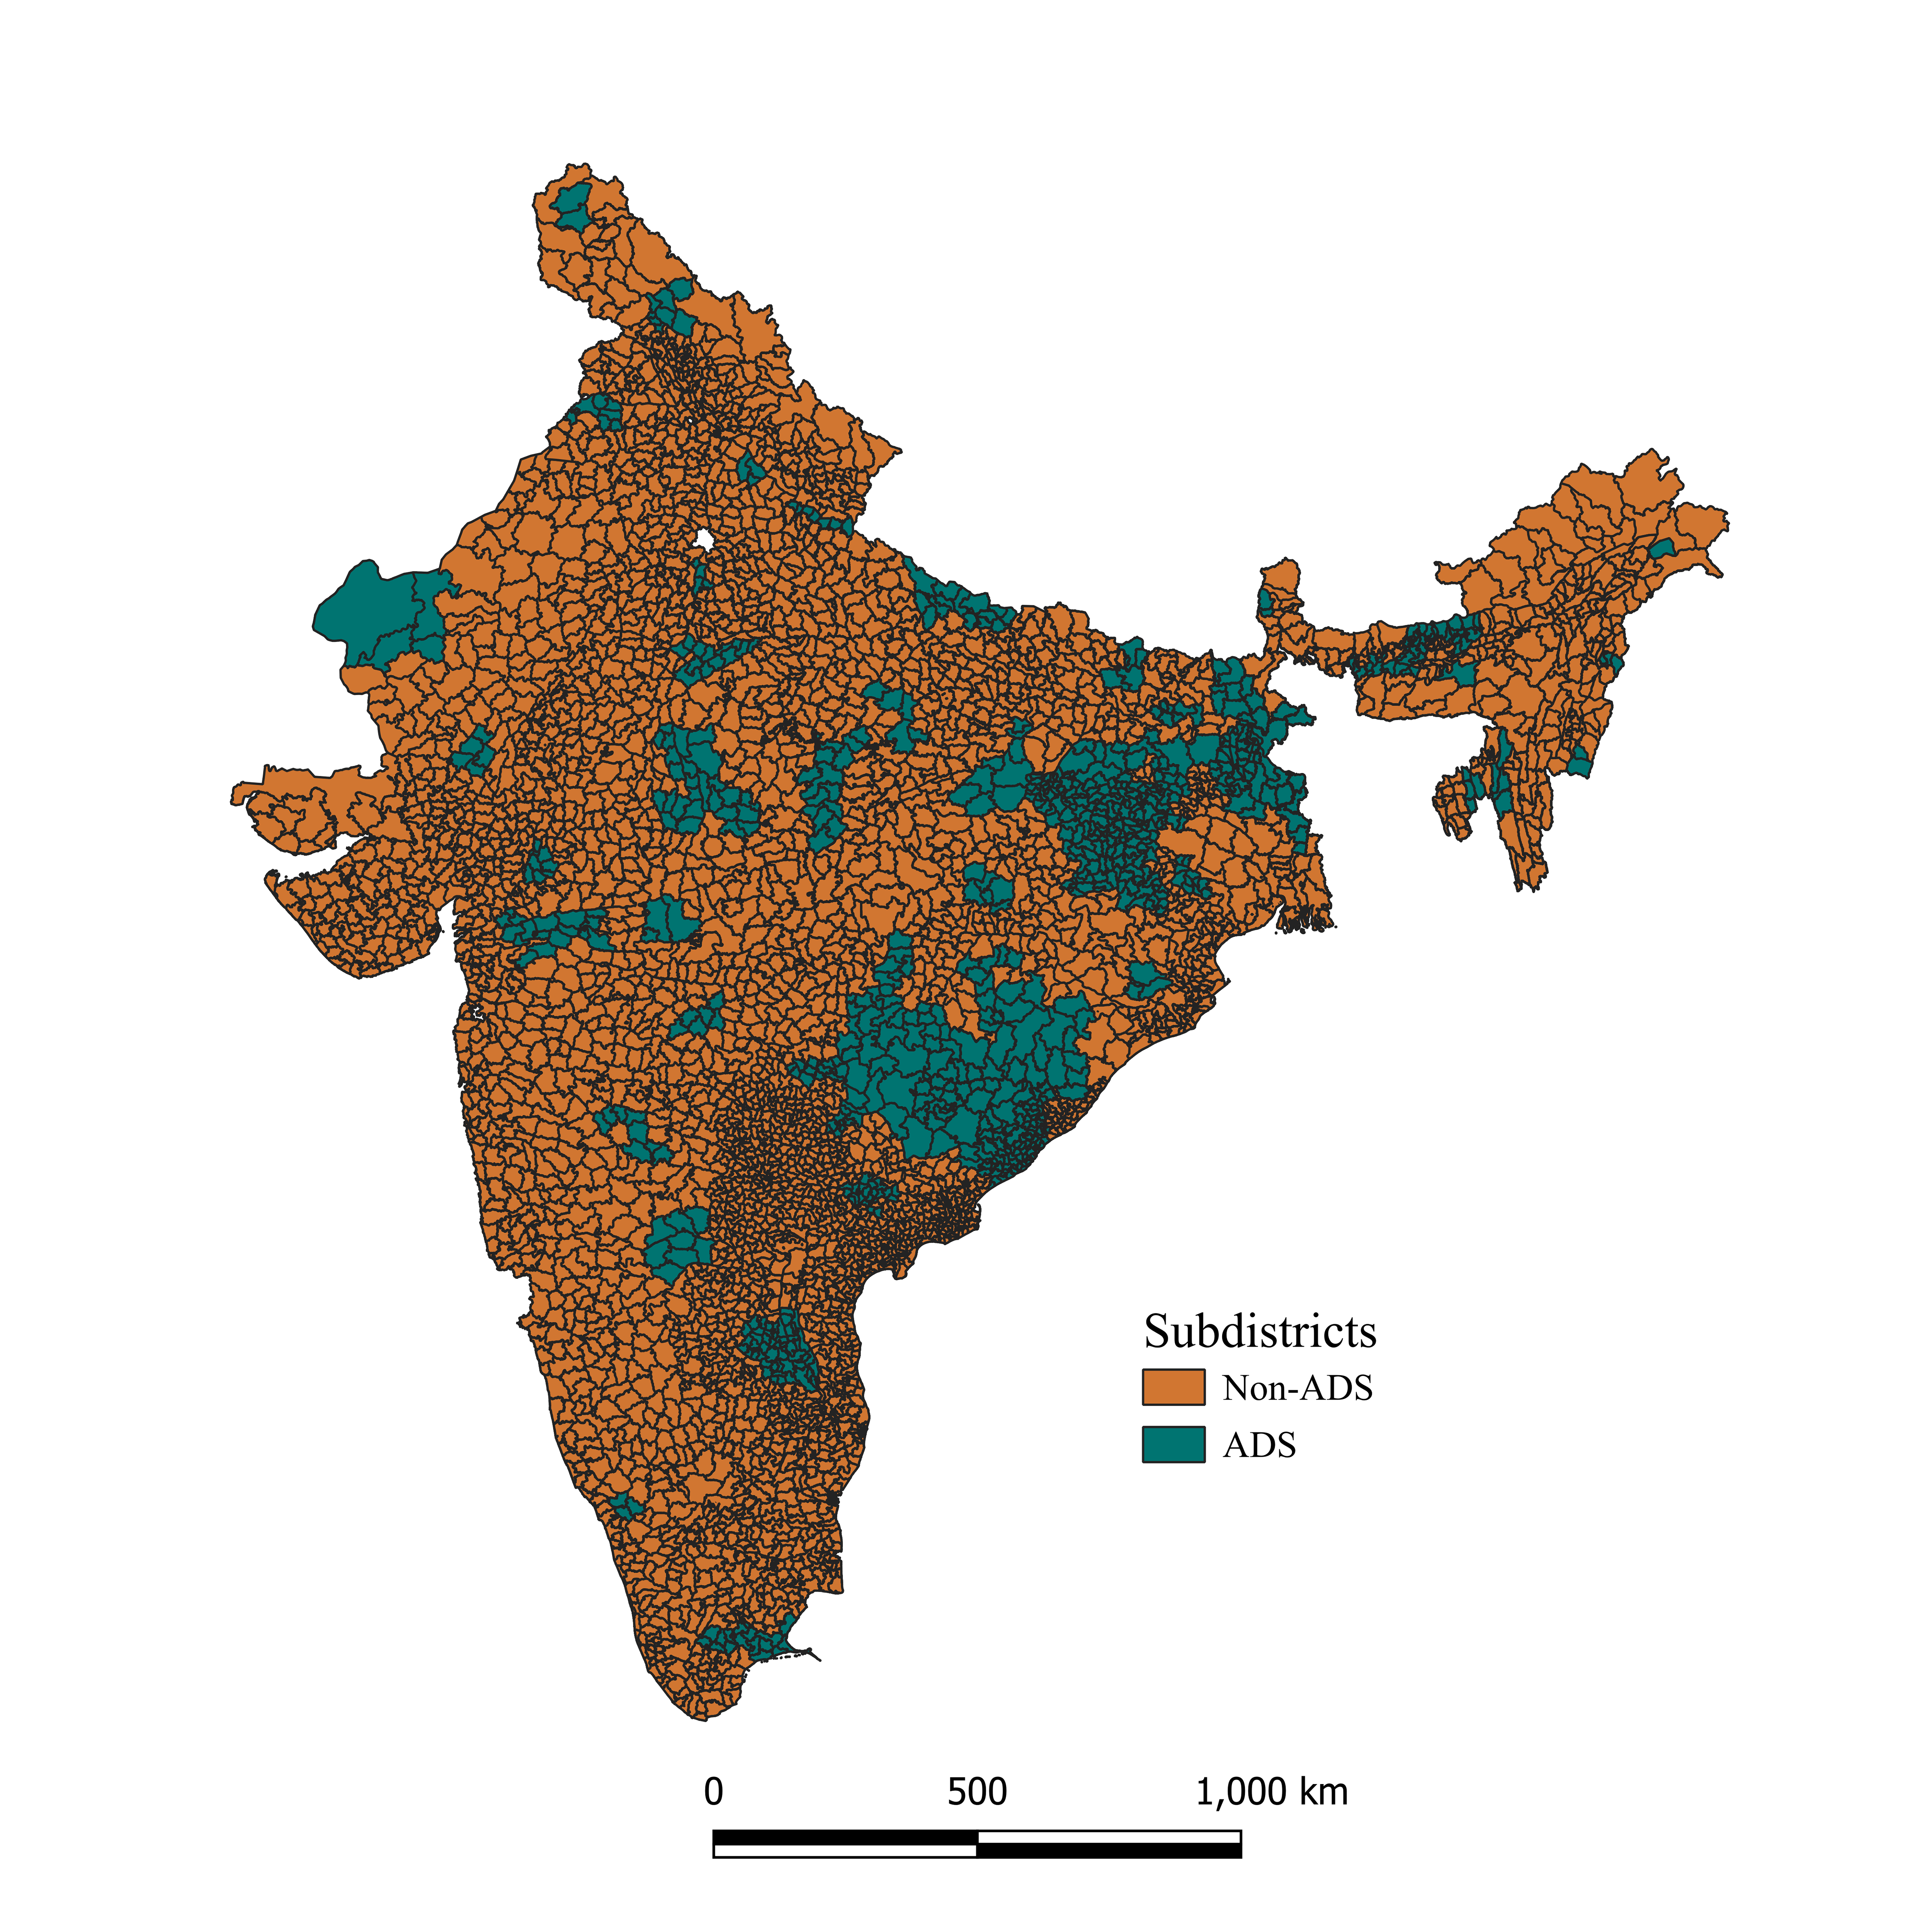
\includegraphics[width=0.5\textwidth]{Images/2_TUT.png}
    \caption{ADS (treated) vs Non-ADS (non-treated) subdistricts}
    \label{fig:tut}
\end{figure}

\subsection{Distance to Cutoff}
A distinctive feature of a regression discontinuity design is the running
variable. While a dummy can indicate whether a unit is treated or not, it is
the running variable which determines how close the unit was to the treatment
cutoff. We employ the more traditionally used Euclidean distance from the
cutoff boundary for each unit as the running variable. The geographic cutoff
was created using the boundary of the treated polygons. This was primarily done
using R and QGIS. The cleaned cutoff boundary is plotted in Figure
\ref{fig:cutoffboundary}. 

\begin{figure}[htbp]
    \centering
    \includegraphics[width=0.5\textwidth]{Images/3C.png}
    \caption{Treatment Cutoff Boundaries}
    \label{fig:cutoffboundary}
\end{figure}

Now, we can use the cutoff boundary to calculate distance to cutoff for each
unit. If the units are points, then the calculation is intuitive. However, for
us the units under study are subdistrict polygons. As a result, we calculate
distance to the cutoff from the centroid of each polygon. We ensured that the
distances to cutoff are positive for the treated units and negative for the
control units.

\subsection{Controls Data} Ideally, the assumption that treatment is
randomly assigned just around the cutoff implies that there is no requirement
for controls in a regression discontinuity design \cite{huntington2021}.
However, in the context of geographic cutoffs these assumptions may not hold
good and potential confounders have to be addressed. The justification for
including controls is not the scope of this section. It will be discussed
later. Here, we shall focus on the data collection aspect of the controls.

To get subdistrict level controls, we used the SHRUG dataset
\cite{shrug2021}. From the SHRUG dataset, we used the Indian population census
data for 2001 (PC01) and 2011 (PC11) to interpolate pre-treatment controls for
the year 2018 \cite{pcindia2011}. For each census year, SHRUG provides a PCA
(Population Census Abstract) directory, a town directory and a village
directory. The SHRUG dataset is designed for the very purpose of spatial
analysis. However, the two shapefiles provided by SHRUG come with their own
problems of either deprecated and incomplete shapefiles. \par \pagebreak

Thus, our master shapefile will remain the one provided by SoI and we will use
SHRUG only for the control variables.

\begin{table}[!htbp]
\centering
\caption{Description of SHRUG variables}
\begin{adjustbox}{width=0.75\textwidth}
\begin{tabular}{|l|l|c|c|}
\hline
\multicolumn{1}{|c|}{\textbf{\begin{tabular}[c]{@{}c@{}}S. \\ No\end{tabular}}} & \multicolumn{1}{c|}{\textbf{Controls}} & \textbf{Description} & \textbf{Directory} \\ \hline
1. & pc11\_pca\_tot\_p & Total population count for 2011 census & PCA \\ \hline
2. & pc11\_pca\_p\_sc & Total Scheduled Castes population & PCA \\ \hline
3. & pc11\_pca\_p\_st & Total Scheduled Tribes population & PCA \\ \hline
4. & pc11\_pca\_p\_lit & Literate Population Total & PCA \\ \hline
5. & pc11\_pca\_tot\_work\_p & Total Workers & PCA \\ \hline
6. & pc11\_vd\_t\_p & Total Population of Village & VD \\ \hline
7. & pc11\_vd\_land\_fores & Forest Area (in Hectares) & VD \\ \hline
8. & pc11\_vd\_area & Total Geographical Area (in Hectares) & VD \\ \hline
9. & pc11\_td\_max\_temp & Maximum Temperature (in C) & TD \\ \hline
10. & pc11\_td\_min\_temp & Minimum Temperature (in C) & TD \\ \hline
11. & pc11\_td\_avg\_rain & Rainfall (mm) & TD \\ \hline
\end{tabular}
\end{adjustbox}
\caption*{\textit{Notes}. Similarly, pc01 for 2001 census.}
\end{table} \par

Since we need to interpolate controls for 2018, the 2001 and 2011 variables
have to be merged. We can use the more granular shrid to merge them and then
aggregate back to the subdistrict level. We remove any observation with NAs in
the desired fields and remove all duplicated shrids (a shrid is a village/town
level data estimation with consistent geometries since 1991) before merging.
The aggregation at the subdistrict level was done by summing all controls
variables for shrids within the same subdistrict. Next, the two subdistrict
level shapefiles (one obtained by this merging exercise and the other SoI
Masterfile) are overlayed and any subdistrict which does not get assigned
controls is dropped from further analysis. \par \pagebreak

Once we have our master shapefile with controls for both 2001 and 2011, we can
use them to interpolate controls for 2018. This was done in the following
manner. First, we calculate the growth rate of the controls between 2001 and
2011:

\begin{equation*}
\textit{Growthrate}_{ij}=\frac{PC11_{ij} - PC01_{ij}}{PC01_{ij}}\times 100
\end{equation*}

Here, $\textit{Growthrate}_{ij}$ is the rate of growth in control $j$ for
subdistrict $i$. Since this is for a period of 10 years, the annual growth rate
is estimated as:

\begin{equation*}
AGR_{ij}=\frac{\textit{Growthrate}_{ij}}{10}
\end{equation*}

Then, controls for 2018 are estimated using the classic population growth formula:

\begin{equation*}
PC18_{ij} = PC11_{ij}\left(1 + \frac{AGR_{ij}}{100}\right)^{7}
\end{equation*}

Once we have the 2018 control values, we use base values (total population or
total area) to convert them into $\%$ shares. Accordingly, the final set of
controls used in this study are presented in the table below.

\begin{table}[htbp]
\centering
\caption{Control variables}
\begin{adjustbox}{width=0.65\textwidth}
\begin{tabular}{|l|l|c|}
\hline
\multicolumn{1}{|c|}{\textbf{\begin{tabular}[c]{@{}c@{}}S. \\ No\end{tabular}}} & \multicolumn{1}{c|}{\textbf{Controls}} & \textbf{Description} \\ \hline
1. & pc18\_sc\_share & Scheduled castes population share \\ \hline
2. & pc18\_st\_share & Scheduled tribes population share \\ \hline
3. & pc18\_lit\_share & Literate population share \\ \hline
4. & pc18\_rural\_share & Rural population share \\ \hline
5. & pc18\_work\_share & Working population share \\ \hline
6. & pc18\_forest\_share & Forest cover share \\ \hline
\end{tabular}
\end{adjustbox}
\end{table}

\subsection{AQI Data}
To measure subdsitrict level air quality, we used PM2.5 pollution from 
the SHRUG dataset \cite{shrug2021}. The name of the variable on the dataset is
Surface PM2.5 and it is described as ``Estimated annual ground-level fine
particulate matter (PM2.5) for 1998-2020 by combining Aerosol Optical Depth
(AOD) retrievals from the NASA MODIS, MISR, and SeaWIFS instruments with the
GEOS-Chem chemical transport model". We have access to the minimum, maximum 
and mean levels of PM2.5 in a subdistrict polygon across 1998 to 2020, however 
for the purpose of this study we will restrict our attention to the mean. \par
Figure \ref{fig:big} plots a heatmap of the subdistrict AQI levels with treatment boundaries.
Any missing values are subdistricts that get lost in the cleaning process.
\begin{figure}[htbp]
\centering
\caption{AQI heatmap with treatment boundaries}
\label{fig:big}
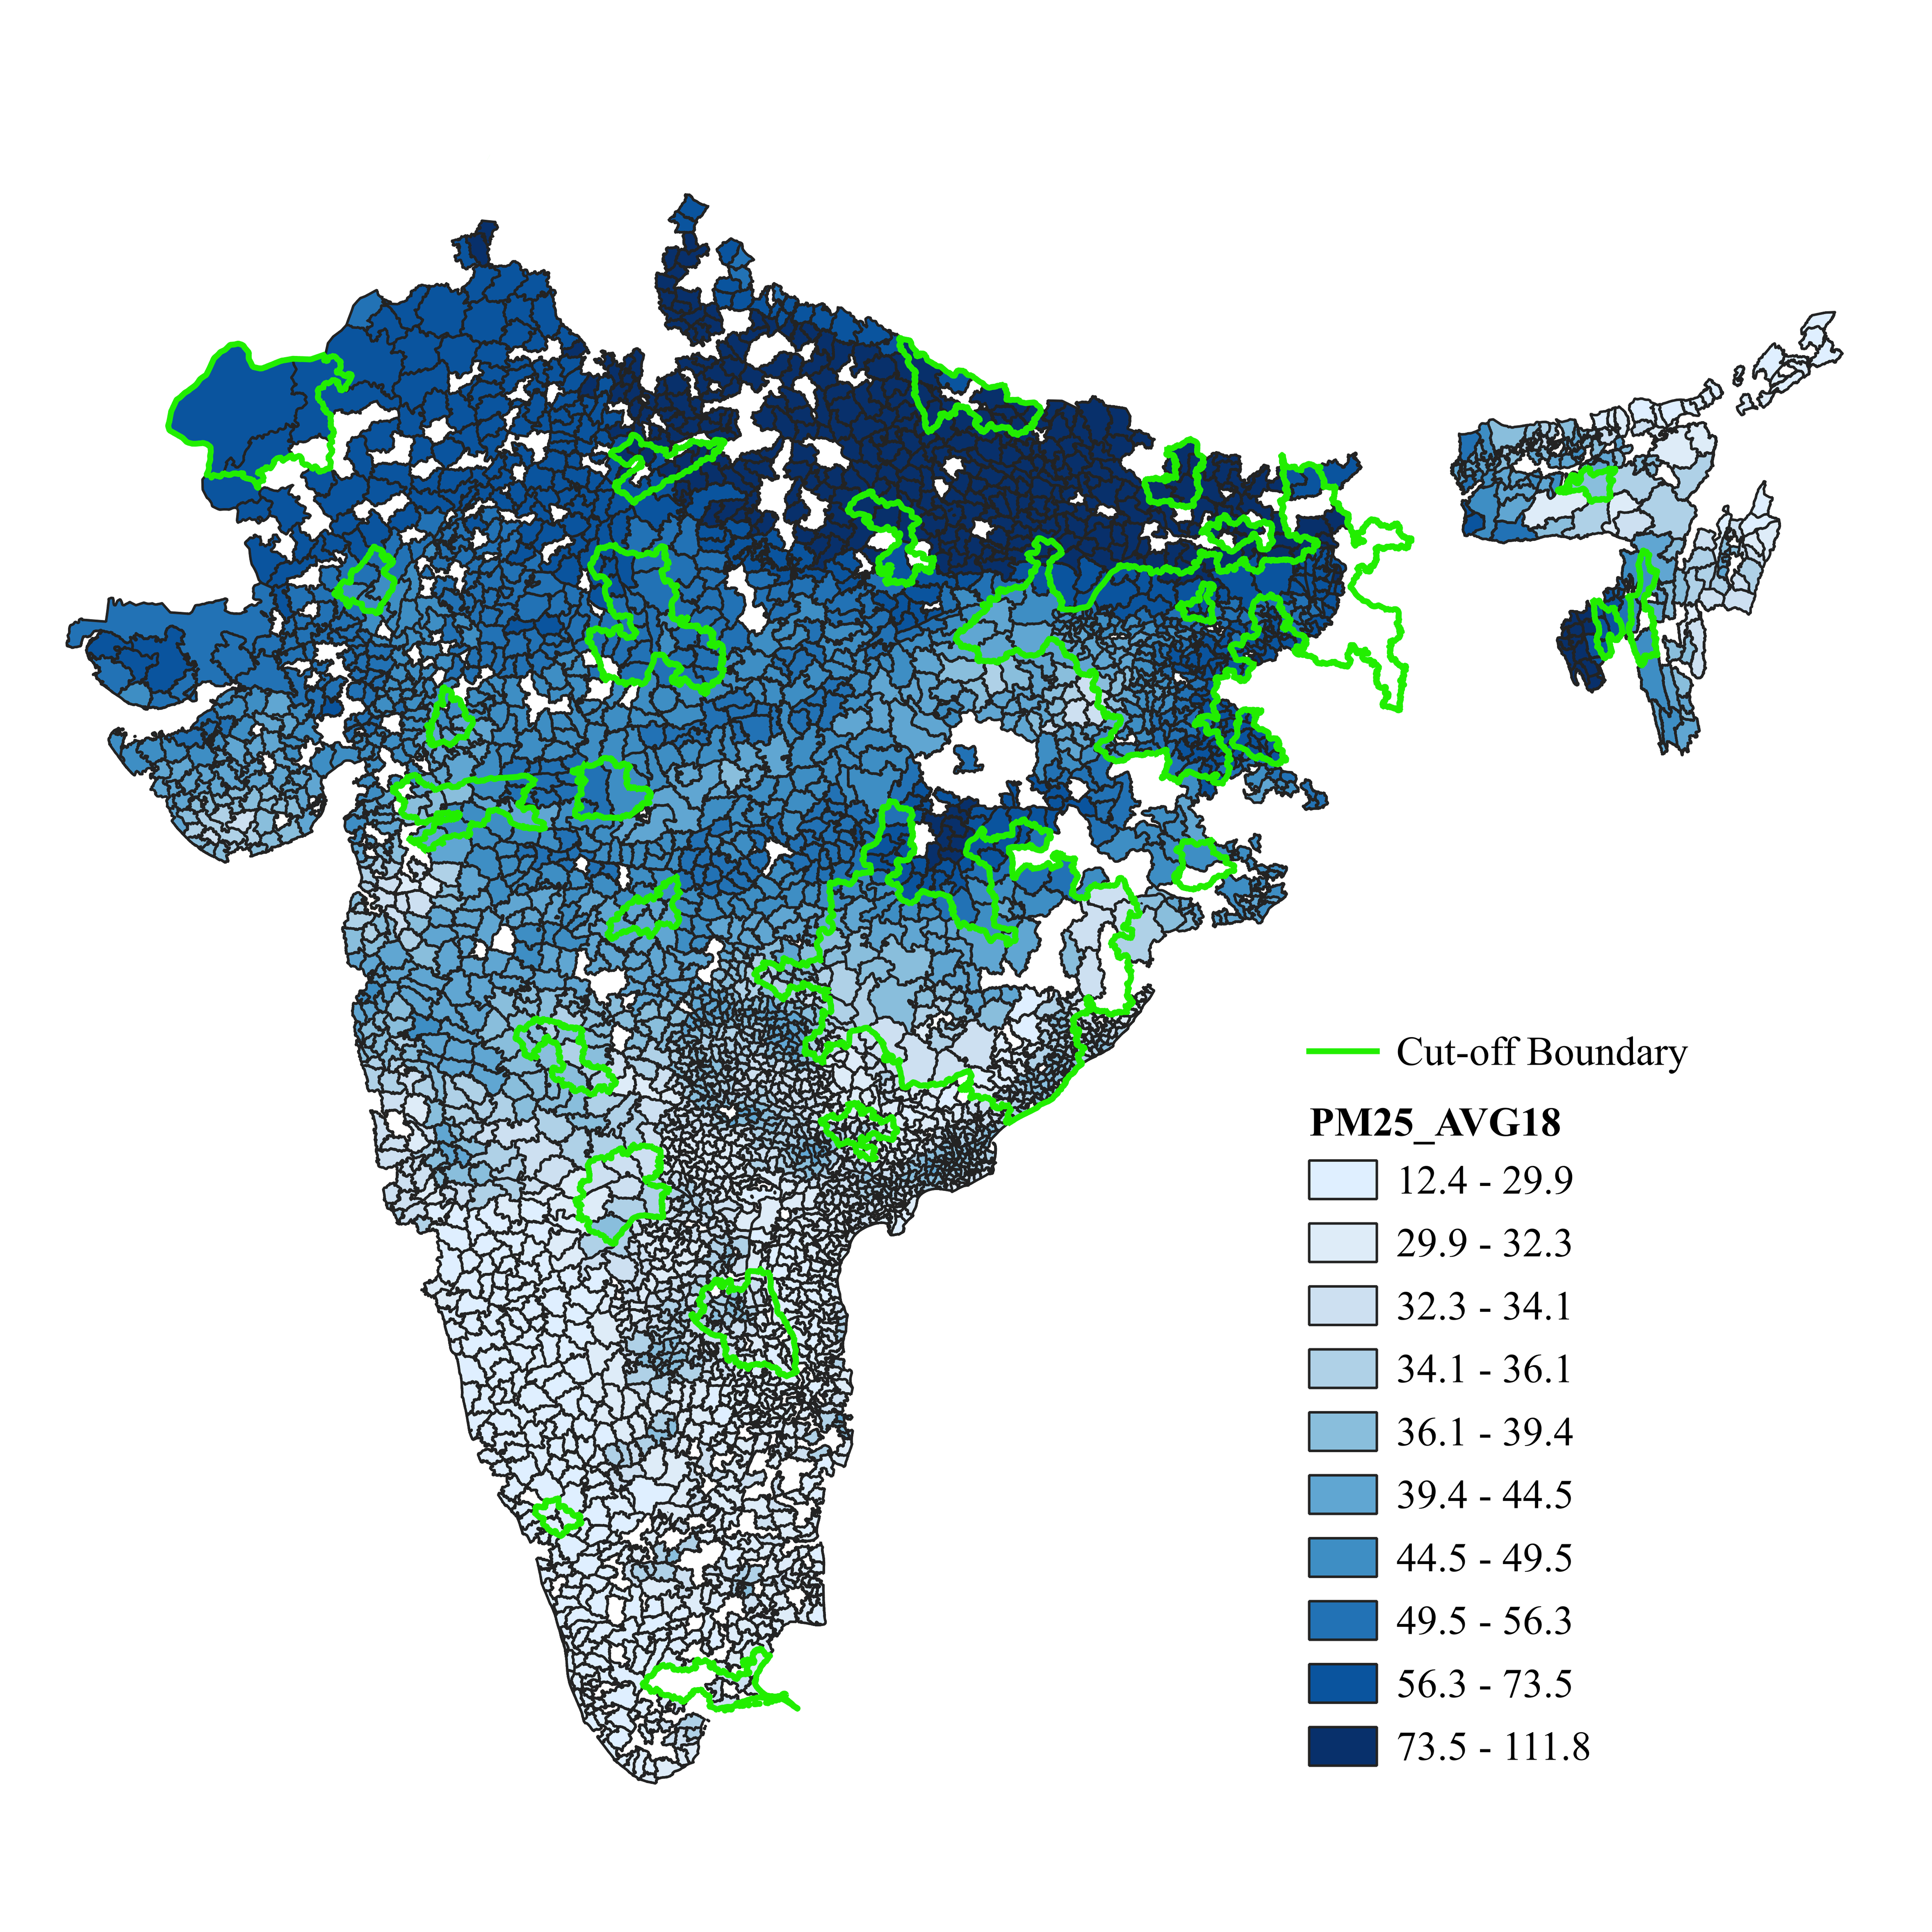
\includegraphics[width=\linewidth]{Controls.png} 
\end{figure}
\newpage
\section{Empirical Strategy}
\subsection{Identifying Strategy}
In this paper, our attempt is to capture the effect of a geographically assigned
treatment on air quality. Though the treatment is assigned at the district level,
we cannot compare differences in AQI across districts as it would suffer
from selection bias. Treating one district over another is a choice made by the
government and not a random selection.
Comparing districts in this regard is plagued by `reverse causality', wherein
it is difficult to isolate the effect of being treated on AQI from the
effect the level of AQI had on the probability of being treated. \par
Therefore, to establish causality we look at the air quality for finer
geographical units namely `Tehsils/Taluks'. The idea is to consider the
district boundaries as a cutoff and compare subdistricts on both sides that are
`just treated' and `just not treated' within a bandwidth. This is called a
regression discontinuity design (RDD), specifically a spatial RDD. Three
recurrent terminologies for this design should be discussed-- running variable,
cutoff and bandwidth. The value of the running variable with respect to the
cutoff determines the treatment status for each unit. The running variable in this study is the distance to
cutoff for each subdistrict, centered at $0$ (cutoff). The bandwidth would be
the equidistant region on both sides of the cutoff within which we will compare
subdistricts. It will be discussed in greater detail in the next section. \par
The identifying assumption of an RDD is that the units close to the cutoff are
`randomly assigned' and cannot choose their own treatment status. If these
conditions are met, we can isolate variation along Treatment $\longrightarrow$
Outcome by controlling all variation in the running variable except for being
above the cutoff \citep{huntington2021}. In our case, being above cutoff is the
same as being treated and resultantly we have a sharp regression discontinuity
design, as shown in the figure below. \par
\begin{figure*}[htbp]
\centering
\caption{DAG}
\begin{tikzpicture}
\node (v0) at (-1.5,0) {Aspirational District};
\node (v1) at (5,0) {ADS scheme};
\node (v2) at (5,2) {AQI};
\node (v3) at (-1.5,3) {Distance to cutoff};
\node (v4) at (5,3) {Z};
\draw [->] (v1) edge (v2);
\draw [->] (v0) edge (v1);
\draw [->] (v3) edge (v0);
\draw [->] (v3) edge (v2);
\draw [->] (v4) edge (v3);
\draw [->] (v4) edge (v2);
\end{tikzpicture}
\end{figure*} \par
Here, Distance to cutoff is the running variable and Aspirational District indicates being above
cutoff. Those who are above the cutoff get the treatment (SRE scheme) which we
suspect affects AQI. Z refers to the unobservable confounders.
\subsection{Model}
In an RDD, the empirical measure for the local average treatment effect (LATE)
is the difference in intercepts of two regressions across the cutoff. As a
result our model takes the following structure--
\begin{equation*}
pm25\_avg18_{i} = \beta_{0} + \beta_{1}A_{i} + \beta_{2}D_{i} + \beta_{3}A_{i}D_{i} + \mu_{i}
\end{equation*}
Here, $pm25\_avg18_{i}$ is the mean PM2.5 of 2018 for subdistrict $i$. $A_{i}$
is a dummy variable indicating treatment
status. It takes value $1$ if subdistrict $i$ lies in the ADS treated area and
$0$ otherwise. $D_{i}$ is the running variable- distance which is centred at
the cutoff. Thus, it reflects the distance from cutoff for subdistrict $i$. The
coefficient of interest is $\beta_{1}$, which is the difference between the
intercepts of two local linear regression just across the cutoff. The above
model is assumed to be a linear regression. However, it is not always the case
that straight lines are a good fit for the data across the cutoff. In this case
we may need to check for nonlinear functional forms like a second-order
polynomial. In that case, our model becomes--
\begin{equation*} 
pm25\_avg18_{i} = \beta_{0} + \beta_{1}A_{i} + \beta_{2}D_{i} +
\beta_{3}{D_{i}}^2 + \beta_{4}A_{i}D_{i} + \beta_{5}A_{i}(D_{i})^2 + \mu_{i}
\end{equation*}
Once again, $\beta_{1}$ is the coefficient of interest and represents the
discontinuity in the two fitted parabolas. Following the recommendations of
\cite{gelman2019}, we do not test for higher order polynomials greater than two.
We use a package in R called \textbf{rdrobust} which allows for
estimation of bias-corrected robust rd estimates \cite{calonico2014}.
The rdrobust package also helps to take the decision regarding bandwidth size
out of the researcher's hands and effectively prevent cherry picking.
It selects that size of bandwidth as optimal which minimizes mean squared error
(MSE). Lastly, since proximity of a subdistrict to the cutoff implies higher
similarity between the controlled and treated units, a weight function is
generally used in spatial regression discontinuity designs. By default,
rdrobust uses a triangularly weighted kernel, i.e., observations right at the
cutoff are given the highest weight and the weights linearly decrease as we
move to either side of the cutoff reaching $0$ at the bandwidth max and min.

\subsection{Controls}
An RDD by the nature of its assumptions does not
require controls. Including controls would imply that we do not expect the
treatment to be randomly assigned around the cutoff. This section will provide
justifications for the use of controls and will discuss the nature of controls
to be included. \par
Our approach to the spatial RDD uses a single running variable (distance to
cutoff) instead of two running variables (latitude and longitude). This
simplification however implies a reduction in dimensionality and a loss of
valuable spatial information. To better understand how this impacts our study,
consider an example. Let there be two subdistricts located far from each other
but equidistant to a cutoff boundary. In the multiple running variable
approach, the lack of proximity between them is evident as we have exact
coordinates. But, in the single running variable approach the two can have the
exact same distance to cutoff. Information regarding their vicinity vis-a-vis
each other is lost \cite{keele2015}. To account for this, we include
pre-treatment controls in the RD estimation. Additionally, adding controls
reduces the unexplained variation which can help increase the precision of the
RD estimates \cite{huntington2021}. \par
To further support the RD assumption, restrictions can be added to the
geographic area in study. Since the treatment is assigned at the district level
we cannot control for them. Otherwise, we would be comparing all treated units
to other treated units and all control units to other control units which is
incorrect. Thus, the largest geographic restriction we can add is at the state
level. This was implemented in two ways. First, we filtered the dataset and ran
our model on each individual state and reported their respective RD estimates.
Second, we considered the entire dataset but included state fixed effects to
report a single RD estimate for all states. In the latter case our
regression equation becomes-
\begin{equation*}
pm25\_avg18_{is} = \beta_{0} + \beta_{1}A_{i} + \beta_{2}D_{i} +
\beta_{3}A_{i}D_{i} + X_{i}\gamma + \lambda_{s} + \mu_{i}
\end{equation*} \par
Here, $X_{i}\gamma$ are a set of subdistrict level controls and $\lambda_{s}$
captures the state fixed effects. Note that these will be omitted when running the
regression individually for each state. \par \pagebreak

\section{Results}

% renumber tables to 4.x
\setcounter{table}{0}
\renewcommand{\thetable}{4.\arabic{table}}

State-wise RD estimates and placebo tests show that the AQI (proxied by the average PM2.5 levels) in 2018 is lower 
for treated subdistricts in Jharkhand. In the aggregated model, no 
statistically significant difference in AQI can be found. For each model run, 
we report the bias-correct robust estimate of $\beta_1$, 95\% confidence interval, 
standard error, robust p-value, number of observations, number of effective observations 
in bandwidth and the data-driven MSE-optimum bandwidth. All standard errors are 
heteroskedasticity robust and the level of clustering will be mentioned (if any). 
This chapter is divided into two sections. The first, discusses the main 
results and the second section provides results from a 
placebo test used to increase the robustness of our estimates for the state where the 
AQI is affected significantly in 2018.

\subsection*{4.1 Main RD estimates}

We begin by estimating the spatial RD with as well as without controls for each 
individual state. Out of the 14 states, the results could not be estimated for Karnataka, Uttar Pradesh, Chattisgarh, Odisha and Assam on account of lower number of observations relative to the number of 
parameters to be estimated. This results in a short ranked matrix.\footnote{More 
variables compared to the number of equations.} For the remaining 9 states, the 
results are presented in Table 4.1.

As suspected, including controls reduces the standard errors for almost all
states, with the exception of Bihar and Madhya Pradesh. Statistically
significant results are found only for Jharkhand. We find that average PM2.5
levels in 2018 are lower in the treated subdistricts of Jharkhand by roughly 19
units in the specification with controls and by about 22 units without
controls. While the conventional RD estimate for several states appears large
or imprecise, the bias-corrected robust estimates indicate that these effects
are not statistically meaningful. For all remaining states, any difference in
PM2.5 levels is likely driven by sampling variability rather than a true
treatment effect. Lastly, although some states experience a reduction in
standard errors after adding controls, the corresponding coefficients also
shrink in magnitude, leaving the overall inference unchanged.

% ---------------------- TABLE 4.1 --------------------------
\begin{table}[ht]\centering
\caption{State-wise Bias-corrected Robust RD Estimates}
\caption*{Outcome variable: Average PM2.5 in 2018}
\begin{adjustbox}{width=0.75\textwidth}
\begin{tabular}{@{\extracolsep{5pt}} lcccccccc} 
\\[-3.5ex]\hline 
\hline \\[-1.8ex] 
 & Estimate & $95\%$ CI & Std. Error & Robust P-Value & Obs & Eff. Obs & Bandwidth & Covs \\ 
\hline \\[-1.8ex] 
ANDHRA PRADESH & $2.125$ & $[-0.772,5.021]$ & $1.478$ & $0.151$ & $635$ & $116$ & $13.515$ & Yes\\ 
ANDHRA PRADESH & $1.382$ & $[-1.813,4.577]$ & $1.630$ & $0.397$ & $635$ & $128$ & $15.345$ & No\\ 
\hline 
BIHAR & $14.087$ & $[-128.410,156.585]$ & $72.704$ & $0.846$ & $79$ & $11$ & $7.035$ & Yes\\ 
BIHAR & $-39.645$ & $[-110.808,31.518]$ & $36.308$ & $0.275$ & $79$ & $5$ & $5.643$ & No\\ 
\hline  
GUJARAT & $3.702$ & $[-14.711,22.115]$ & $9.394$ & $0.694$ & $201$ & $47$ & $36.846$ & Yes\\ 
GUJARAT & $-0.989$ & $[-24.325,22.346]$ & $11.906$ & $0.934$ & $201$ & $47$ & $34.969$ & No\\ 
\hline 
\textbf{JHARKHAND} & $\textbf{-18.790}$ & $\textbf{[-35.527,-2.054]}$ &
$\textbf{8.539}$ & $\textbf{0.028}$ & $\textbf{256}$ & $\textbf{17}$ &
$\textbf{4.398}$ & \textbf{Yes}\\ 
JHARKHAND & $ -22.381$ & $ [-40.013,-4.749]$ & $ 8.996$ & $ 0.013$ & $ 256$ & $ 43$ & $ 6.602$ & No\\  
\hline 
MADHYA PRADESH & $3.868$ & $[-4.513,12.250]$ & $4.277$ & $0.366$ & $259$ & $77$ & $24.041$ & Yes\\ 
MADHYA PRADESH & $6.142$ & $[-2.170,14.454]$ & $4.241$ & $0.148$ & $259$ & $72$ & $21.989$ & No\\ 
\hline 
MAHARASHTRA & $0.746$ & $[-17.722,19.214]$ & $9.423$ & $0.937$ & $329$ & $53$ & $15.824$ & Yes\\ 
MAHARASHTRA & $-2.357$ & $[-28.844,24.129]$ & $13.514$ & $0.862$ & $329$ & $54$ & $16.327$ & No\\ 
\hline 
MIZORAM & $8.251$ & $[1.925,14.578]$ & $3.228$ & $0.011$ & $16$ & $15$ & $124.220$ & Yes\\ 
MIZORAM & $23.682$ & $[14.480,32.884]$ & $4.695$ & $0.000$ & $16$ & $15$ & $124.220$ & No\\ 
\hline 
RAJASTHAN & $29.610$ & $[-25.449,84.670]$ & $28.092$ & $0.292$ & $230$ & $45$ & $17.098$ & Yes\\ 
RAJASTHAN & $31.702$ & $[-26.159,89.562]$ & $29.521$ & $0.283$ & $230$ & $63$ & $25.969$ & No\\ 
\hline 
TELANGANA & $2.924$ & $[-17.674,23.522]$ & $10.509$ & $0.781$ & $429$ & $23$ & $5.165$ & Yes\\ 
TELANGANA & $-13.303$ & $[-50.241,23.636]$ & $18.847$ & $0.480$ & $429$ & $21$ & $4.833$ & No\\ 
\hline 
\end{tabular} 
\end{adjustbox}
\end{table}

Next, we estimate the spatial RD model for the full dataset by pooling all
subdistricts together and including state fixed effects. The aggregated
estimate is not statistically significant, as shown in Table 4.2. This is
expected, since only one state - Jharkhand, exhibits a significant treatment
effect, and the remaining states show estimates close to zero. When these
heterogeneous state-level effects are combined, the overall impact naturally
averages out. For inference, \textit{rdrobust} already reports
heteroskedasticity-robust nearest-neighbour standard errors (based on the three
closest units), which effectively behaves like subdistrict-level clustering.
Therefore, clustering at the subdistrict level does not change the results, and
we do not report it separately. Since treatment effects differ across states,
clustering at the state level is more appropriate. Although state-clustered
standard errors are slightly smaller than the unclustered ones, they are still
not small enough to make the pooled estimate statistically significant.

% ---------------------- TABLE 4.2 (correct place) --------------------------
\begin{table}[ht]\centering
\caption{Aggregated Bias-corrected Robust RD Estimates}
\caption*{Outcome variable: Total PM2.5 in 2018}
\begin{adjustbox}{width=0.75\textwidth}
\begin{tabular}{@{\extracolsep{5pt}} lcccccccc} 
\\[-3.5ex]\hline 
\hline \\[-1.8ex] 
 & Estimate & $95\%$ CI & Std. Error & Robust P-Value & Obs & Eff. Obs & Bandwidth & Covs \\ 
\hline \\[-1.8ex] 
ALL STATES & $1.829$ & $[-1.561,5.220]$ & $1.730$ & $0.290$ & $3456$ & $889$ & $20.572$ & Yes\\ 
ALL STATES & $-1.916$ & $[-17.619,13.787]$ & $8.012$ & $0.811$ & $3456$ & $1194$ & $30.659$ & No\\ 
\hline \\[-1.8ex] 
\end{tabular} 
\end{adjustbox}
\caption*{\textit{Notes}. Standard errors are clustered by state.}
\end{table}

\subsection*{4.2 Placebo test}

As discussed earlier, many schemes and policies that already existed were
implemented more effectively under the Aspirational Districts Programme in
2018. However, to establish that the significant results we observe for
Jharkhand are caused by the 2018 intervention and not the effect of any
previously existing treatment, we conducted a placebo test which checks for
discontinuity using 2018 boundaries for “dummy’’ pre-2018 PM2.5 data (2017). If
the novel treatments did not exist before 2018, then there should be no
difference in PM2.5 across the control and treated units. The same was
confirmed and results are presented in Table 4.3.

% ---------------------- TABLE 4.3 --------------------------
\begin{table}[ht]\centering
  \caption{Placebo Test} 
	\caption*{Outcome variable: PM2.5 in 2017 (before policy implementation)}
\begin{adjustbox}{width=0.75\textwidth}
\begin{tabular}{@{\extracolsep{5pt}} lcccccccc} 
\\[-3.5ex]\hline 
\hline \\[-1.8ex] 
 & Estimate & $95\%$ CI & Std. Error & Robust P-Value & Obs & Eff. Obs & Bandwidth & Covs \\ 
\hline \\[-1.8ex] 
JHARKHAND & $-17.297$ & $[-36.163,1.568]$ & $9.626$ & $0.072$ & $256$ & $29$ & $5.261$ & Yes\\ 
\hline \\[-1.8ex] 
\end{tabular} 
\end{adjustbox}
\caption*{\textit{Notes}. Standard errors are heteroskedasticity robust.}
\end{table}

To understand why Jharkhand displays a statistically significant improvement in
PM2.5 levels after the launch of the Aspirational Districts Scheme (ADS), it is
important to consider how districts were selected and how the scheme interacts
with the state’s baseline conditions. The ADS identifies districts using a
composite deprivation index covering five sectors: health, education,
agriculture, financial inclusion and basic infrastructure. Jharkhand performs
poorly across several of these dimensions, particularly in basic
infrastructure, which resulted in 19 out of its 24 districts being classified
as aspirational. Because the ADS measures incremental progress relative to a
district’s starting point, states beginning from very low baselines tend to
show rapid improvements once interventions are introduced. Jharkhand’s low
initial levels therefore created substantial scope for early gains, reflected
in the immediate reductions in PM2.5 in 2018. This is consistent with the sharp
rise in its Delta Ranking, where Ranchi moved from rank 106 to rank 10 within a
few months of the scheme’s launch.

Jharkhand’s administrative and political context further strengthened this
effect. As a state affected by Left-Wing Extremism (LWE), it already operated
within a strong centre–state coordination framework, facilitating tighter
monitoring, targeted resource flows and better alignment with national
priorities. This allowed the ADP’s model of convergence, competition and
collaboration to operate more effectively compared to many other states.
Improvements in basic services, digital monitoring, Anganwadi strengthening,
nutrition interventions and early action under the state’s Clean Air Action
Plans were implemented with greater coherence and speed. The combination of
extensive district coverage, very low starting conditions, strong centre–state
collaboration in LWE-affected regions and high administrative convergence
explains why Jharkhand alone displays a statistically significant discontinuity
in PM2.5 levels.

\section{Conclusion}
Our results indicate that the Aspirational Districts Programme had a
statistically significant impact on air quality only in Jharkhand, where
treated subdistricts experienced an improvement of roughly 18.8 units in PM2.5
in 2018. This aligns with the state’s low baseline conditions, extensive
coverage under the programme, and rapid early improvements documented in the
Delta Rankings. The aggregate results provide evidence of a dual
mechanism: development interventions can generate short-term pollution through
construction and economic activity, yet simultaneously reduce pollution through
improved public services, institutional strengthening, and cleaner
infrastructure.

At the same time, the study has limitations, particularly regarding potential
spatial spillovers and the use of Euclidean rather than network-based
distances. Future work can enhance robustness by analysing outcomes at finer
geographies such as villages or towns, and by incorporating a two–running
variable design to better validate RD assumptions. Understanding how
development shapes environmental outcomes remains essential for designing
policies that promote growth while safeguarding public health.


\bibliographystyle{apalike}
\bibliography{references} \pagebreak

\appendix
\section{Additional Tables}
\hbadness=10000
\begin{table}[!htbp]
\centering
\caption{State-wise $2018$ ADS Districts}
\vspace{10pt}
\begin{adjustbox}{width=0.85\textwidth}
\begin{tabular}{|c|l|c|p{10cm}|}
\hline
\textbf{S. No} & \textbf{State} & \textbf{No. of Districts} & \textbf{Districts} \\ \hline

1 & Karnataka & 2 & Raichur, Yadgir. \\ \hline

2 & Andhra Pradesh & 3 & Vizianagaram, Visakhapatnam, Cuddapah. \\ \hline

3 & Telangana & 3 & Khammam, Jayashankar Bhoopalapally, Kumuram Bheem (Asifabad). \\ \hline

4 & Uttar Pradesh & 8 & Chitrakoot, Fatehpur, Bahraich, Shravasti, Balrampur, Siddharthnagar, Chandauli, Sonbhadra. \\ \hline

5 & Rajasthan & 5 & Dholpur, Karauli, Jaisalmer, Sirohi, Baran. \\ \hline

6 & Jharkhand & 19 & Garhwa, Chatra, Giridih, Godda, Sahebganj, Pakur, Bokaro, Lohardaga,
Purbi Singhbhum, Palamu, Latehar, Hazaribagh, Ramgarh, Dumka,
Ranchi, Khunti, Gumla, Simdega, Pashchimi Singhbhum. \\ \hline

7 & Chhattisgarh & 10 & 
Korba, Rajnandgaon, Mahasamund, Uttar Bastar Kanker, Bastar,
Narayanpur, Dakshin Bastar Dantewada, Bijapur, Sukma, Kondagaon. \\ \hline

8 & Madhya Pradesh & 8 & 
Chhatarpur, Damoh, Barwani, Rajgarh, Vidisha, Guna,
Singrauli, Khandwa (East Nimar). \\ \hline

9 & Mizoram & 1 & Mamit. \\ \hline

10 & Maharashtra & 4 & Nandurbar, Washim, Gadchiroli, Osmanabad. \\ \hline

11 & Bihar & 13 & Sitamarhi, Araria, Purnia, Katihar, Muzaffarpur, Begusarai,
Khagaria, Banka, Sheikhpura, Aurangabad, Gaya, Nawada, Jamui. \\ \hline

12 & Gujarat & 2 & Dahod, Narmada. \\ \hline

13 & Odisha & 10 & Dhenkanal, Gajapati, Kandhamal, Balangir, Nuapada, Kalahandi,
Rayagada, Nabarangpur, Koraput, Malkangiri. \\ \hline

14 & Assam & 7 & 
Dhubri, Goalpara, Barpeta, Hailakandi, Baksa, Darrang, Udalguri. \\ \hline

15 & Arunachal Pradesh & 1 & Namsai. \\ \hline

16 & Jammu \& Kashmir & 2 & Kupwara, Baramulla. \\ \hline

17 & Punjab & 2 & Moga, Firozpur. \\ \hline

18 & Sikkim & 1 & West Sikkim District. \\ \hline

19 & Tamil Nadu & 2 & Virudhunagar, Ramanathapuram. \\ \hline

20 & Manipur & 1 & Chandel. \\ \hline

21 & Meghalaya & 1 & Ri Bhoi. \\ \hline

22 & Nagaland & 1 & Kiphire. \\ \hline

23 & Tripura & 1 & Dhalai. \\ \hline

24 & Uttarakhand & 2 & Udham Singh Nagar, Haridwar. \\ \hline

25 & West Bengal & 5 & 
Dakshin Dinajpur, Malda, Murshidabad, Birbhum, Nadia. \\ \hline

\multicolumn{2}{|r|}{\textbf{Total}} & \textbf{117} & \\ \hline

\end{tabular}
\end{adjustbox}
\caption*{\textit{Source-} NITI Aayog}
\end{table}


\end{document}
